% Daily gain of an orbiting clock over a clock on the ground, against orbit
% radius (Earth's rotation ignored). Rates in microseconds per day:
%   height  H = K (1 - R/r),   speed  S = -(K/2)(R/r),   net  N = K (1 - 3R/2r),
% with K = GM/(c^2 R) x 86400 s x 1e6 = 60.146 and R = 6371 km.
% Numbers checked in checks/rev1_quoted_numbers.py.
\documentclass[tikz,border=1pt]{standalone}
% Shared preamble for the standalone figures: the book's fonts, palette and
% drawing styles. Figures are drawn at their final printed size. A column is
% 3.35in (241pt) wide; a figure across both columns is 7in (505pt) wide.

\usepackage[T1]{fontenc}
\usepackage{newpxtext}
\usepackage[varbb]{newpxmath}
\usepackage[semibold,scale=0.95,lining]{sourcesanspro}
\usepackage{xcolor}
% Palette shared by the book and by the standalone figures in figures/src.
% One main hue (blue), one accent (orange), and a few roles used sparingly.

\definecolor{seblue}{HTML}{1D5B8F}    % headings, worked examples, main curves
\definecolor{seblueDark}{HTML}{123E63}
\definecolor{seorange}{HTML}{DC7A26}  % thought experiments, light and light cones
\definecolor{seteal}{HTML}{1F8577}    % checks, travellers and ships
\definecolor{sered}{HTML}{C0392B}     % negative energy, tension, violations
\definecolor{seviolet}{HTML}{5E548E}  % going deeper
\definecolor{sesand}{HTML}{8C6A3F}    % history
\definecolor{segray}{HTML}{6B7480}    % axes, guides, secondary labels
\definecolor{selight}{HTML}{D5DAE1}   % grids and faint rules

\usepackage{siunitx}
\usepackage{fontawesome5}
\usepackage{tikz}
\usetikzlibrary{arrows.meta,calc,positioning,decorations.pathreplacing,
  decorations.markings,shapes.geometric,fadings,shadings,patterns,3d,
  intersections,backgrounds}
\usepackage{pgfplots}
\pgfplotsset{compat=1.18}
\usepgfplotslibrary{fillbetween,groupplots,colormaps}

\tikzset{
  >={Latex[length=2.1mm,width=1.4mm]},
  every picture/.style={line cap=round, line join=round},
  lbl/.style={font=\sffamily\footnotesize, text=black!85},
  smalllbl/.style={font=\sffamily\scriptsize, text=black!75},
  guide/.style={segray, line width=0.4pt},
  axisline/.style={segray, line width=0.5pt, -{Latex[length=1.7mm,width=1.1mm]}},
  light/.style={seorange, line width=0.9pt},
  lightdash/.style={seorange, line width=0.9pt, dash pattern=on 3pt off 2pt},
  ship/.style={seteal, line width=1.4pt},
  cone/.style={fill=seorange!22, draw=seorange!85!black, line width=0.35pt},
}

\pgfplotsset{
  se axis/.style={
    axis lines=left,
    axis line style={segray, line width=0.5pt, -{Latex[length=1.6mm,width=1.1mm]}},
    tick style={segray, line width=0.4pt},
    major tick length=2.5pt,
    tick label style={font=\sffamily\scriptsize, text=black!75},
    label style={font=\sffamily\footnotesize, text=black!85},
    every axis plot/.append style={line width=1.1pt},
    legend style={font=\sffamily\scriptsize, draw=none, fill=none},
    scaled ticks=false,
    xticklabel={\sansnum{\tick}}, yticklabel={\sansnum{\tick}},
  },
}

% Numbers in figures are set in the sans-serif text font, with a true minus.
\sisetup{mode=text, reset-text-family=false, reset-text-series=false,
  reset-text-shape=false, drop-zero-decimal, group-minimum-digits=5}
% Tick values arrive as long decimals (1.5000000000); parse them first.
\newcommand{\sansnum}[1]{\begingroup\pgfkeys{/pgf/fpu=false}%
  \pgfmathparse{1*(#1)}\num{\pgfmathresult}\endgroup}

\begin{document}
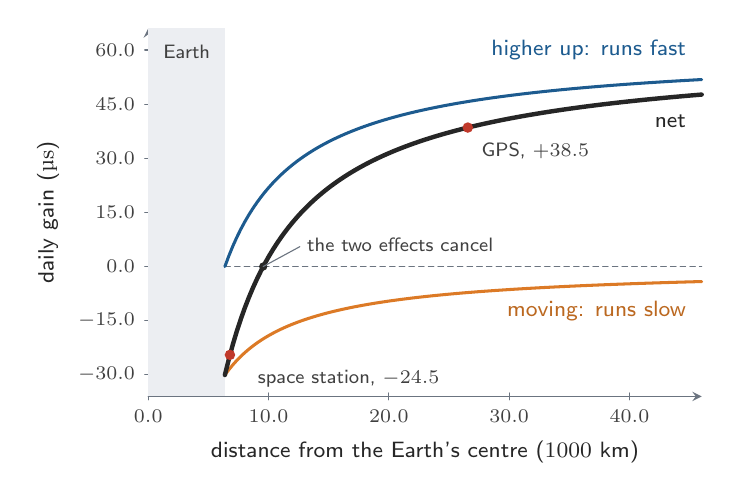
\begin{tikzpicture}
\begin{axis}[
  se axis,
  width=245pt, height=178pt,
  xmin=0, xmax=46, ymin=-36, ymax=66,
  xtick={0,10,20,30,40}, ytick={-30,-15,0,15,30,45,60},
  xlabel={distance from the Earth's centre (\num{1000} km)},
  ylabel={daily gain (\si{\micro\second})},
  clip=false,
  axis x line=bottom, axis y line=left,
]
% Earth's surface and the zero line
\fill[selight!45] (axis cs:0,-36) rectangle (axis cs:6.371,66);
\node[smalllbl, anchor=north] at (axis cs:3.2,64) {Earth};
\draw[guide, dash pattern=on 2pt off 1.5pt] (axis cs:6.371,0) -- (axis cs:46,0);

% the two effects and their sum
\addplot[seblue, domain=6.371:46, samples=120] {60.146*(1 - 6.371/x)};
\addplot[seorange, domain=6.371:46, samples=120] {-30.073*6.371/x};
\addplot[black!85, line width=1.6pt, domain=6.371:46, samples=120] {60.146*(1 - 1.5*6.371/x)};

% direct labels
\node[lbl, text=seblue, anchor=south east, align=right] at (axis cs:45.5,54.5)
  {higher up: runs fast};
\node[lbl, text=black!85, anchor=north east] at (axis cs:45.5,44.8) {net};
\node[lbl, text=seorange!85!black, anchor=north east, align=right] at (axis cs:45.5,-7)
  {moving: runs slow};

% where the effects cancel
\fill[black!85] (axis cs:9.557,0) circle (1.5pt);
\draw[guide] (axis cs:9.557,0) -- (axis cs:12.6,5.5);
\node[smalllbl, anchor=west, align=left] at (axis cs:12.4,6) {the two effects cancel};

% satellites
\fill[sered] (axis cs:6.791,-24.49) circle (1.9pt);
\node[smalllbl, anchor=west] at (axis cs:8.3,-31) {space station, \num{-24.5}};
\fill[sered] (axis cs:26.56,38.51) circle (1.9pt);
\node[smalllbl, anchor=north west] at (axis cs:26.9,36.8) {GPS, \num[print-implicit-plus]{+38.5}};
\end{axis}
\end{tikzpicture}
\end{document}
